\section{DeepSeek-R1}

\begin{frame}{DeepSeek-R1: Why It Made the News}
  \begin{figure}
    \centering
    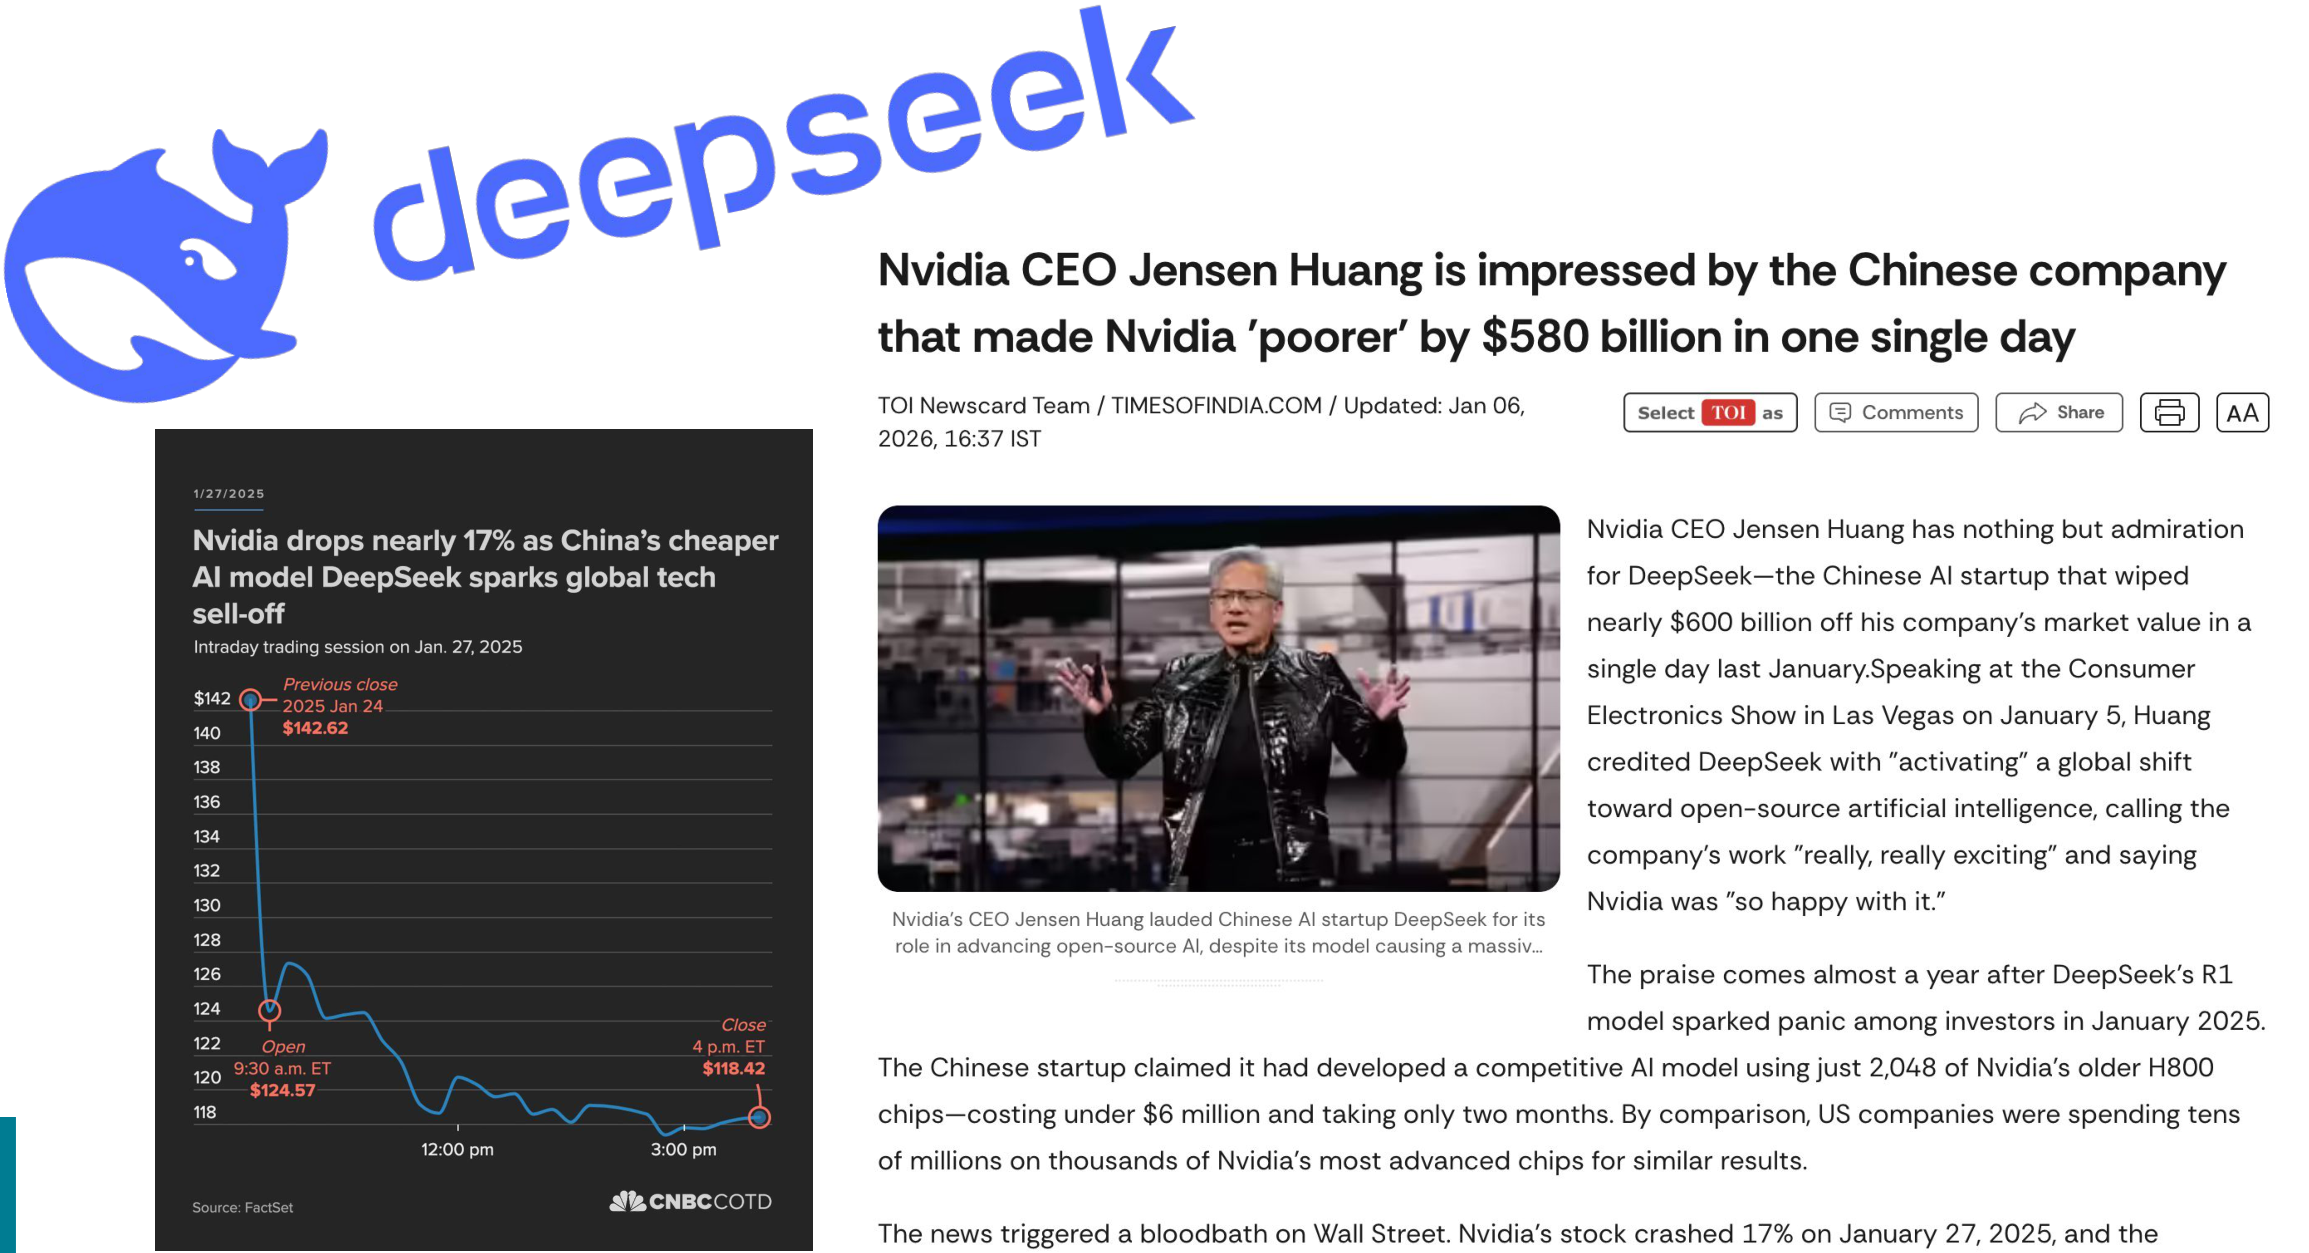
\includegraphics[width=\textwidth,height=0.78\textheight,keepaspectratio]{images/lrm-grpo/deepseek_r1_nvidia_market_reaction.png}
    \caption*{Source: Stanford CS224N, Lecture 12 (Choi, 2026); assembled from screenshots of CNBC (chart, data: FactSet) and The Times of India.}
  \end{figure}
\end{frame}

\begin{frame}{DeepSeek-R1: Training Pipeline Overview}
  \begin{figure}
    \centering
    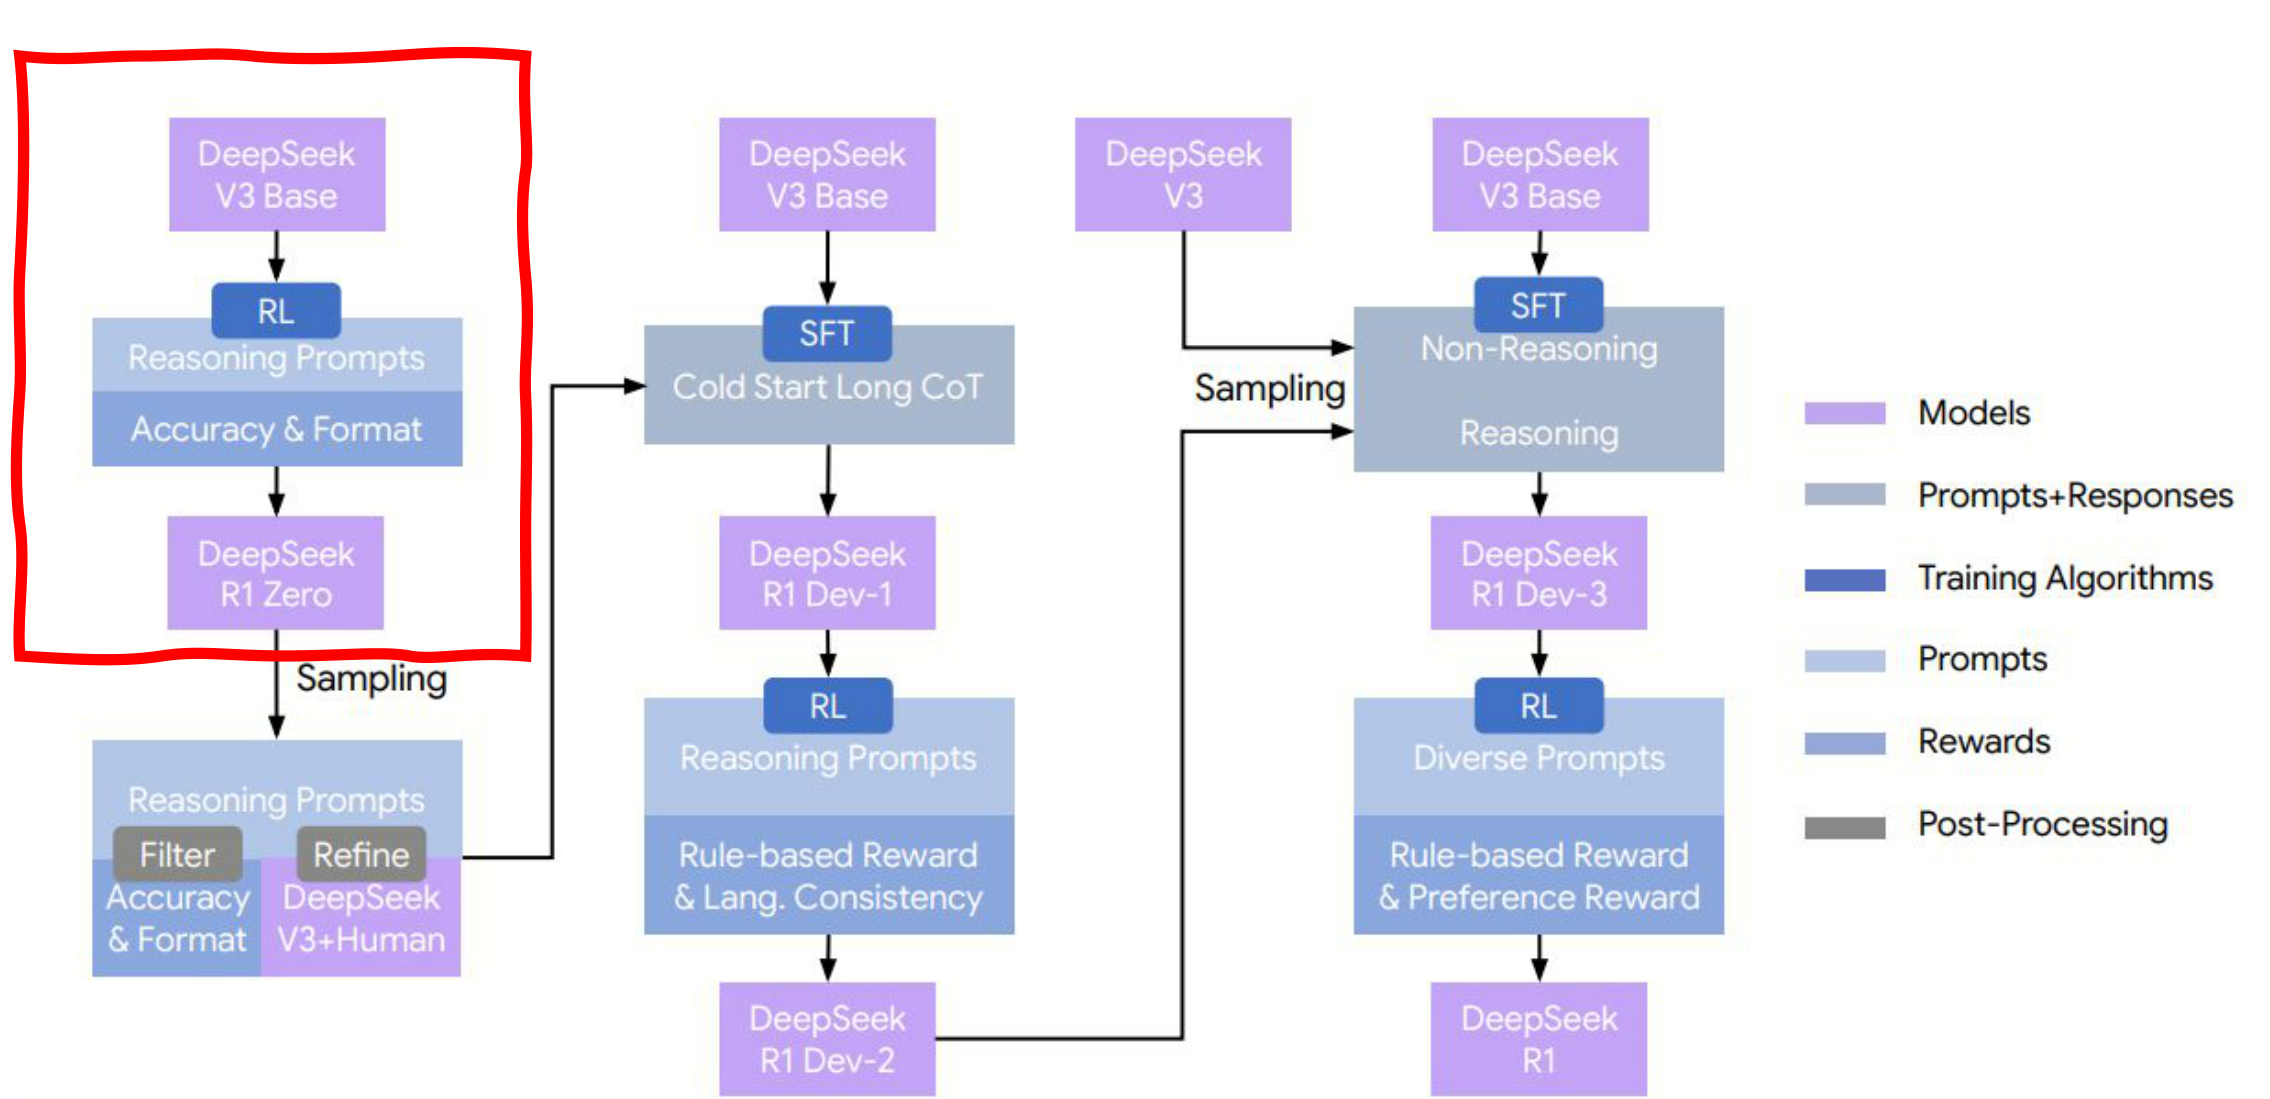
\includegraphics[width=\textwidth,height=0.80\textheight,keepaspectratio]{images/lrm-grpo/deepseek_r1_pipeline_overview_highlighted.png}
    \caption*{The highlighted branch is R1-Zero: pure RL on the base model. Figure: DeepSeek-AI (2025), \href{https://arxiv.org/abs/2501.12948}{arXiv:2501.12948}, Fig.~2; red highlight added in Stanford CS224N, Lecture 12 (Choi, 2026).}
  \end{figure}
\end{frame}

\begin{frame}{DeepSeek-R1-Zero: The ``Aha Moment''}
  \begin{figure}
    \centering
    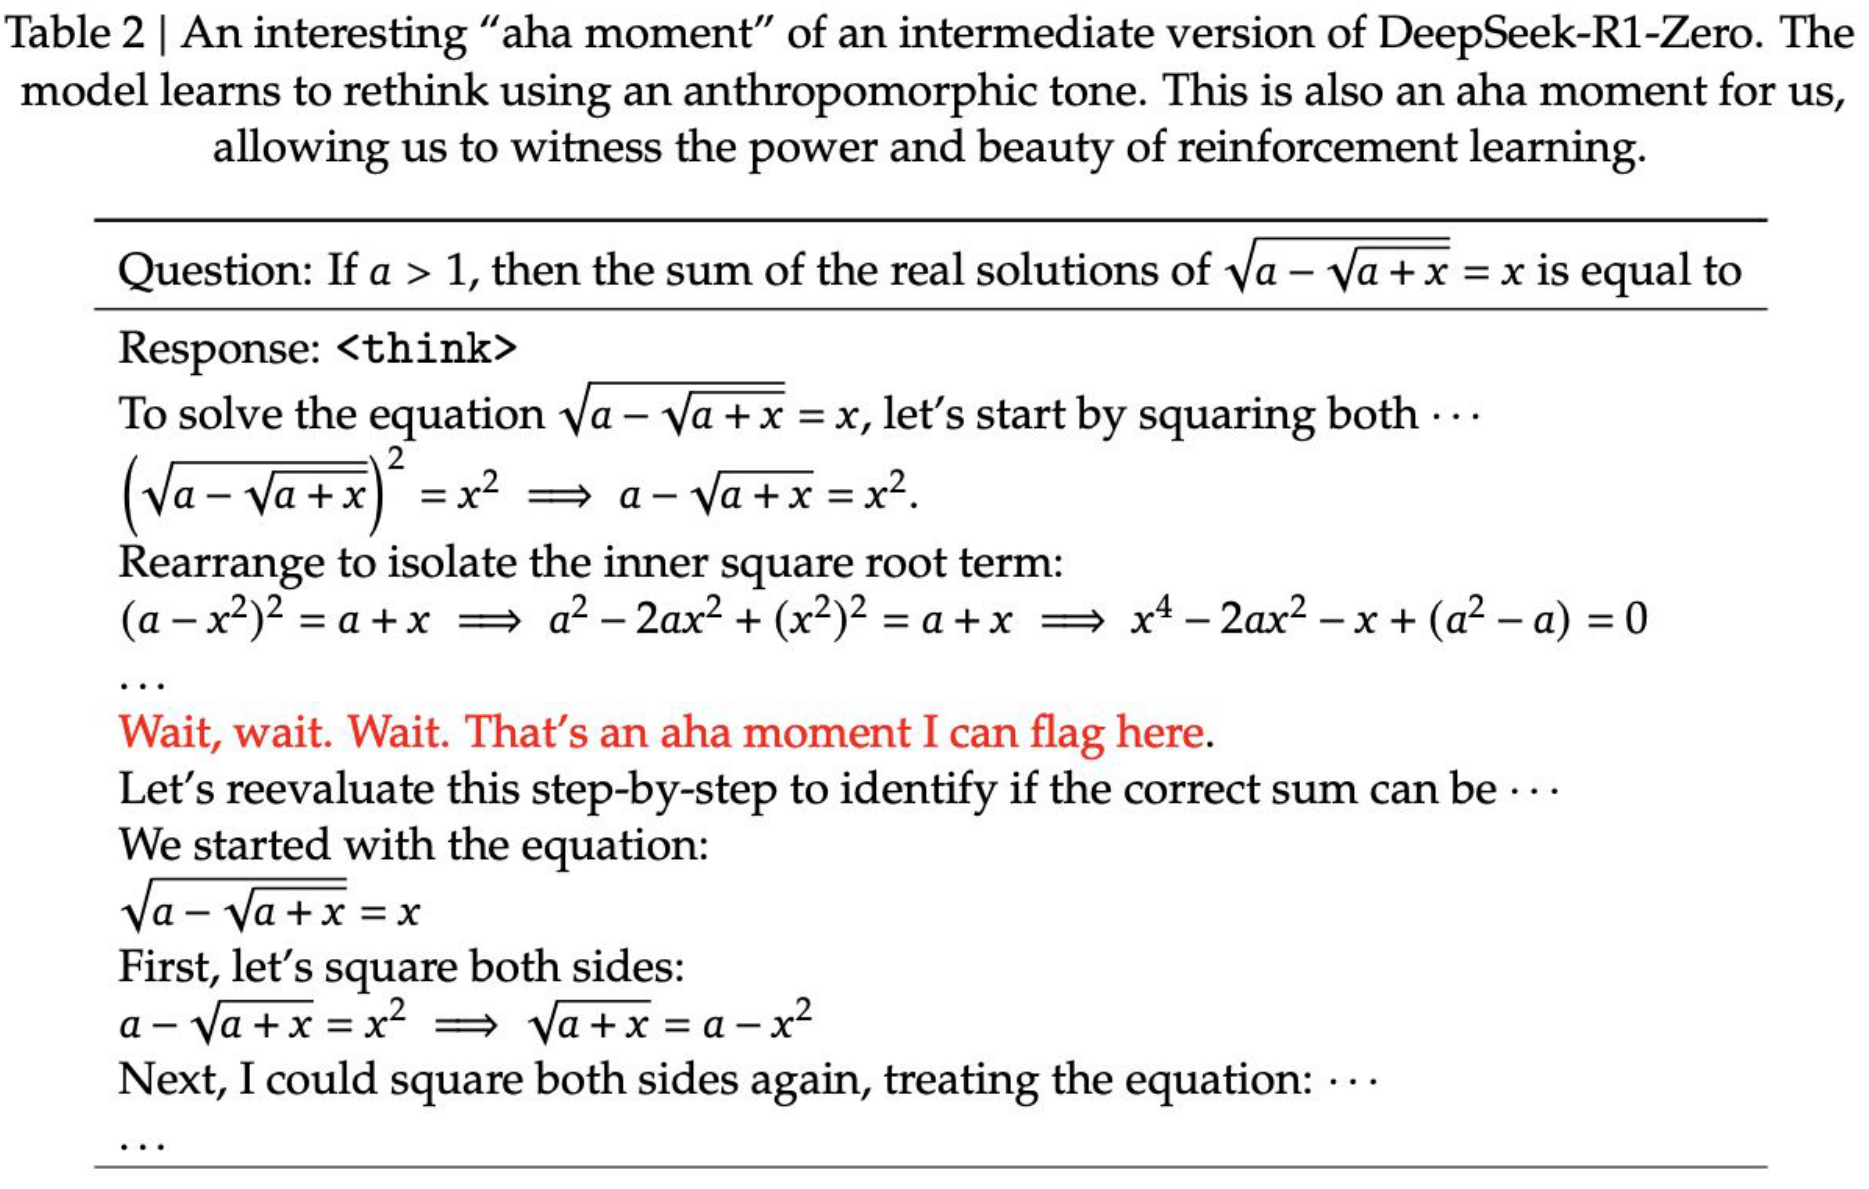
\includegraphics[width=\textwidth,height=0.78\textheight,keepaspectratio]{images/lrm-grpo/deepseek_r1_zero_aha_moment_example.png}
    \caption*{Source: DeepSeek-AI (2025), \href{https://arxiv.org/abs/2501.12948}{arXiv:2501.12948}, Table~2; via Stanford CS224N, Lecture 12 (Choi, 2026).}
  \end{figure}
\end{frame}

\begin{frame}{Reward for R1-zero: keeping it simple}
  \begin{figure}
    \centering
    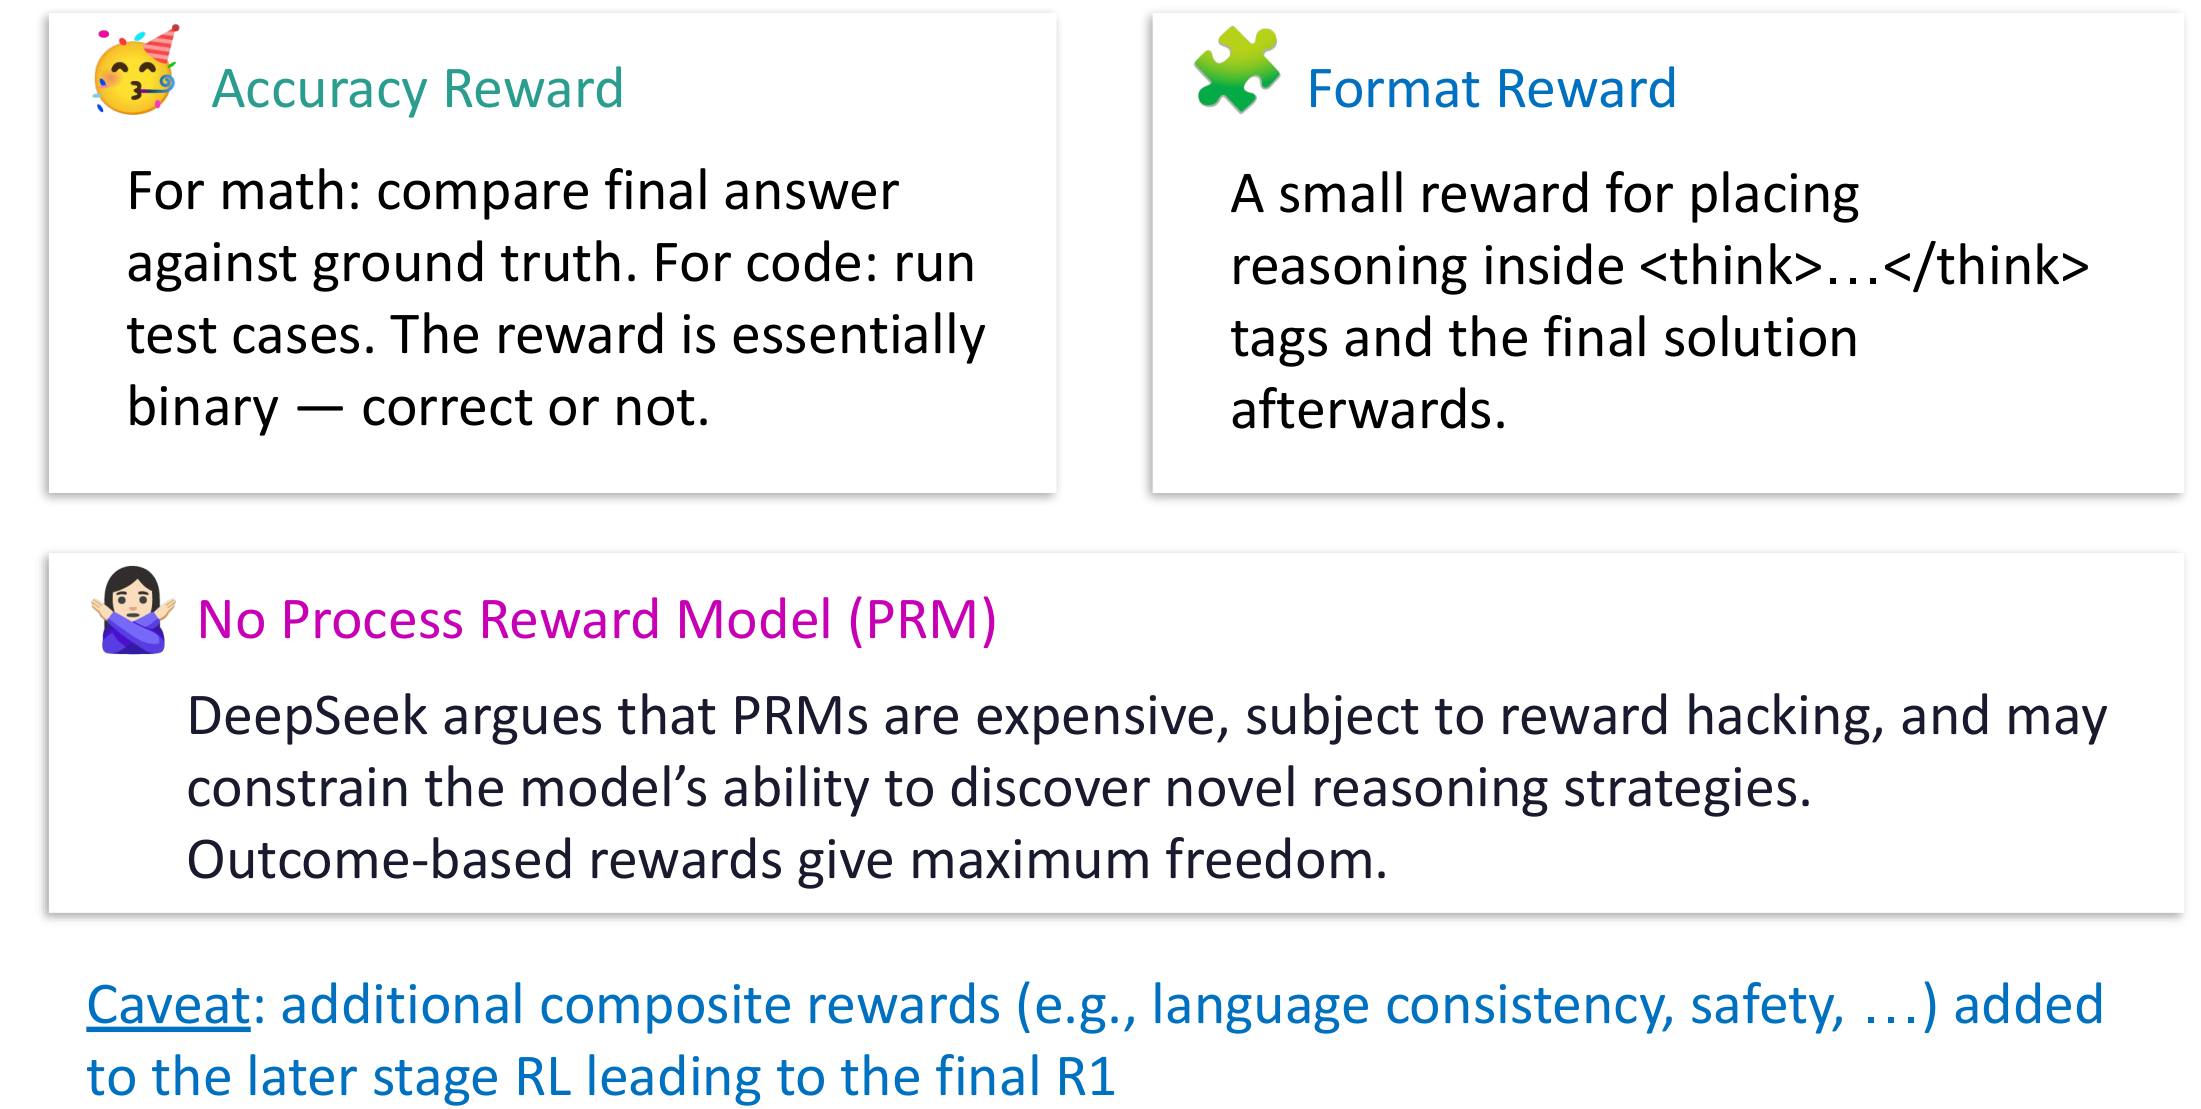
\includegraphics[width=\textwidth,height=0.86\textheight,keepaspectratio]{images/lrm-grpo/deepseek_r1_zero_reward_design.png}
    \caption*{Source: Stanford CS224N, Lecture 12 (Choi, 2026).}
  \end{figure}
\end{frame}

\begin{frame}{Emergent reasoning capabilities}
  \begin{figure}
    \centering
    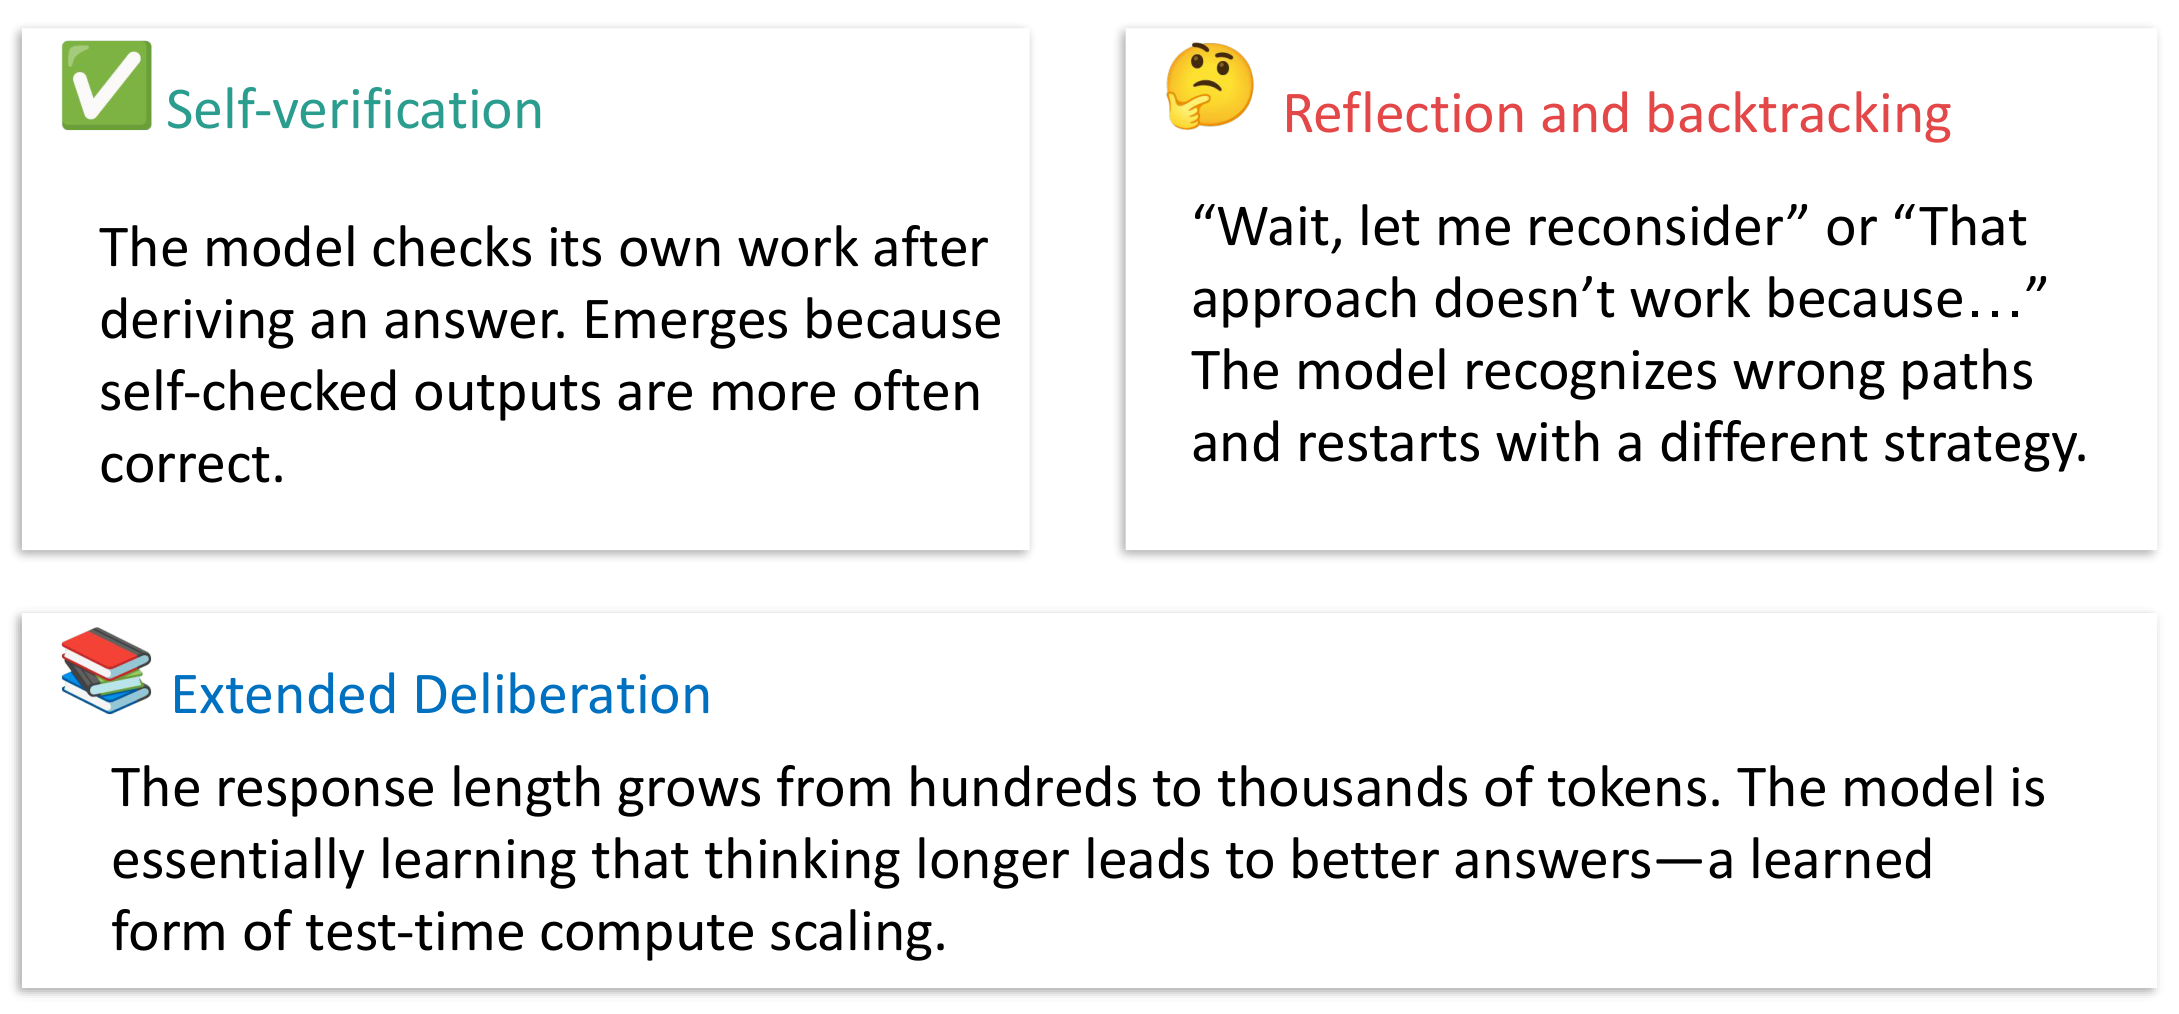
\includegraphics[width=\textwidth,height=0.86\textheight,keepaspectratio]{images/lrm-grpo/deepseek_r1_zero_emergent_capabilities.png}
    \caption*{Source: Stanford CS224N, Lecture 12 (Choi, 2026).}
  \end{figure}
\end{frame}

\begin{frame}{Emergent undesirable characteristics of R1-Zero}
  \begin{figure}
    \centering
    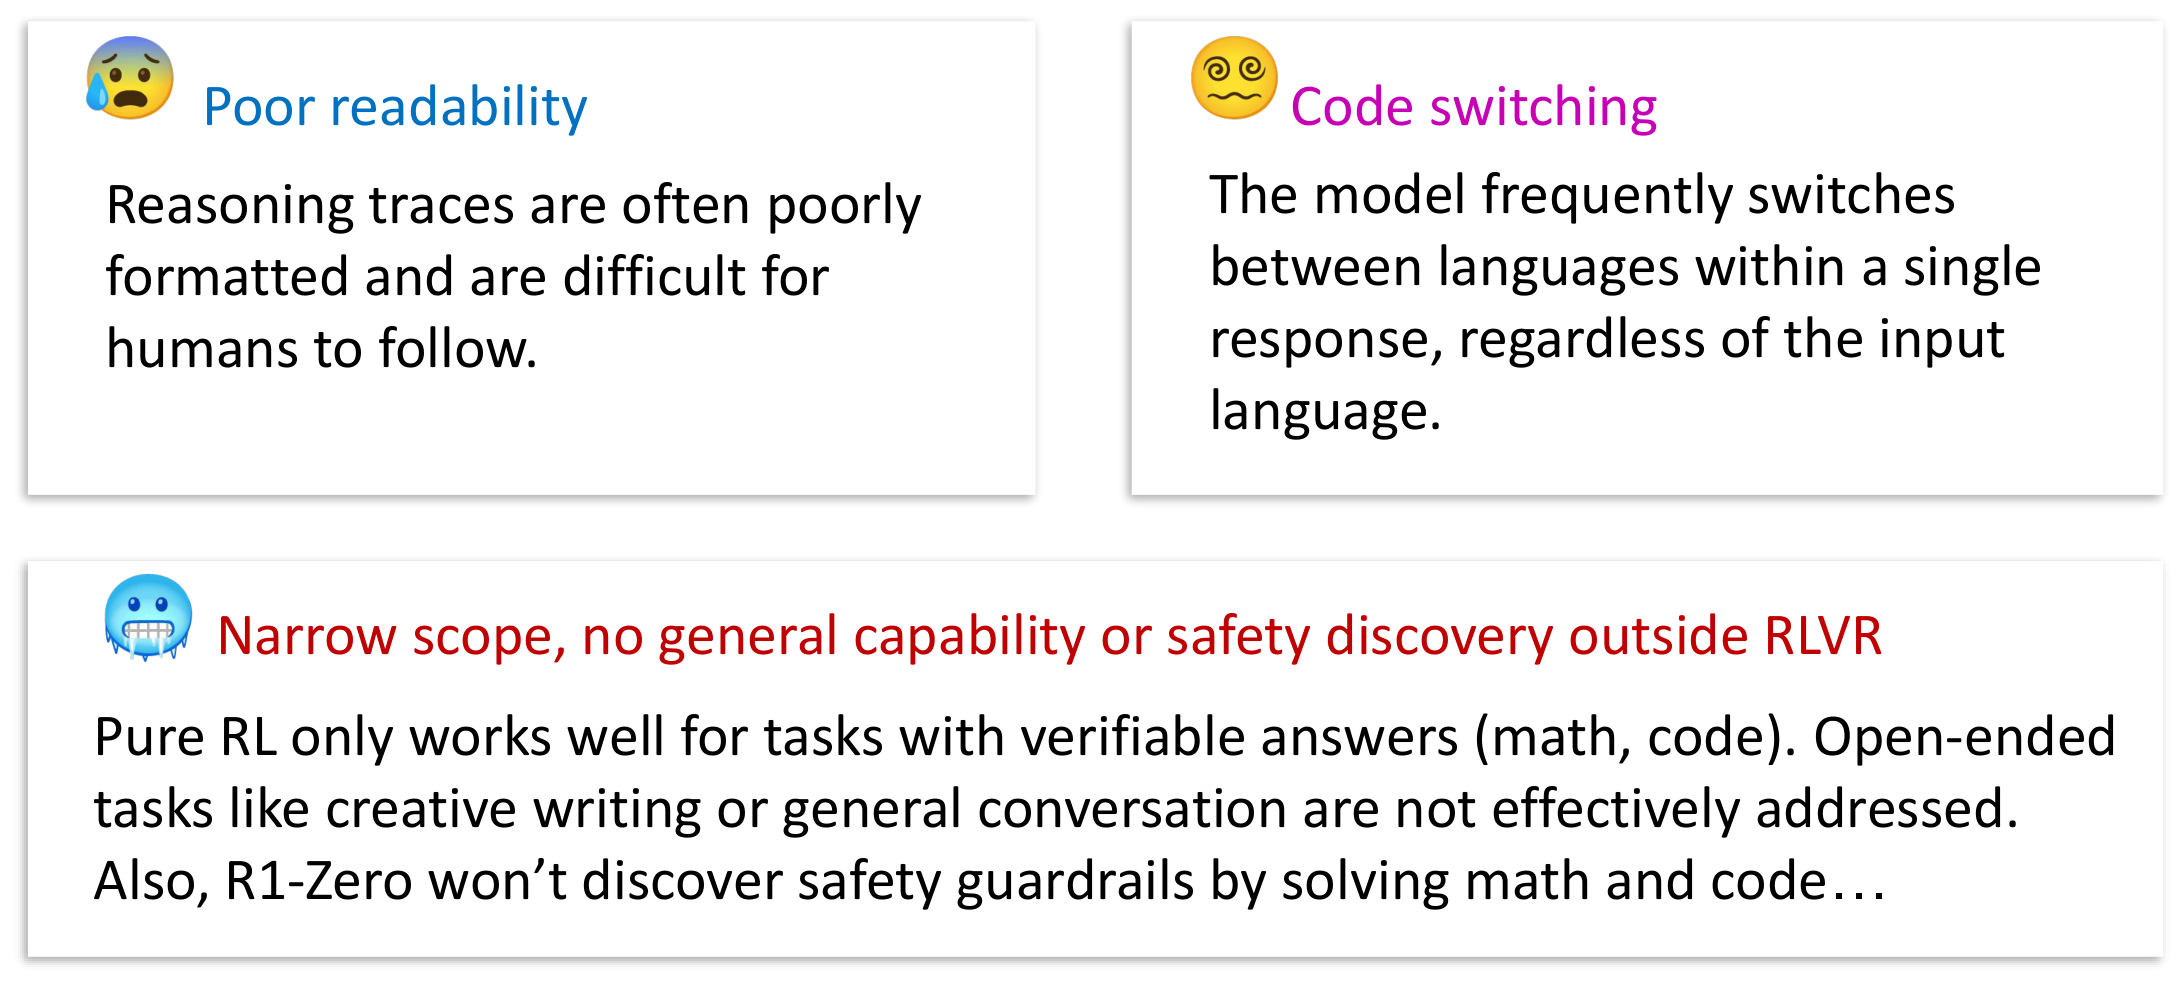
\includegraphics[width=\textwidth,height=0.86\textheight,keepaspectratio]{images/lrm-grpo/deepseek_r1_zero_undesirable_characteristics.png}
    \caption*{Source: Stanford CS224N, Lecture 12 (Choi, 2026).}
  \end{figure}
\end{frame}

\begin{frame}{DeepSeek-R1: The Full Four-Stage Pipeline}
  \begin{figure}
    \centering
    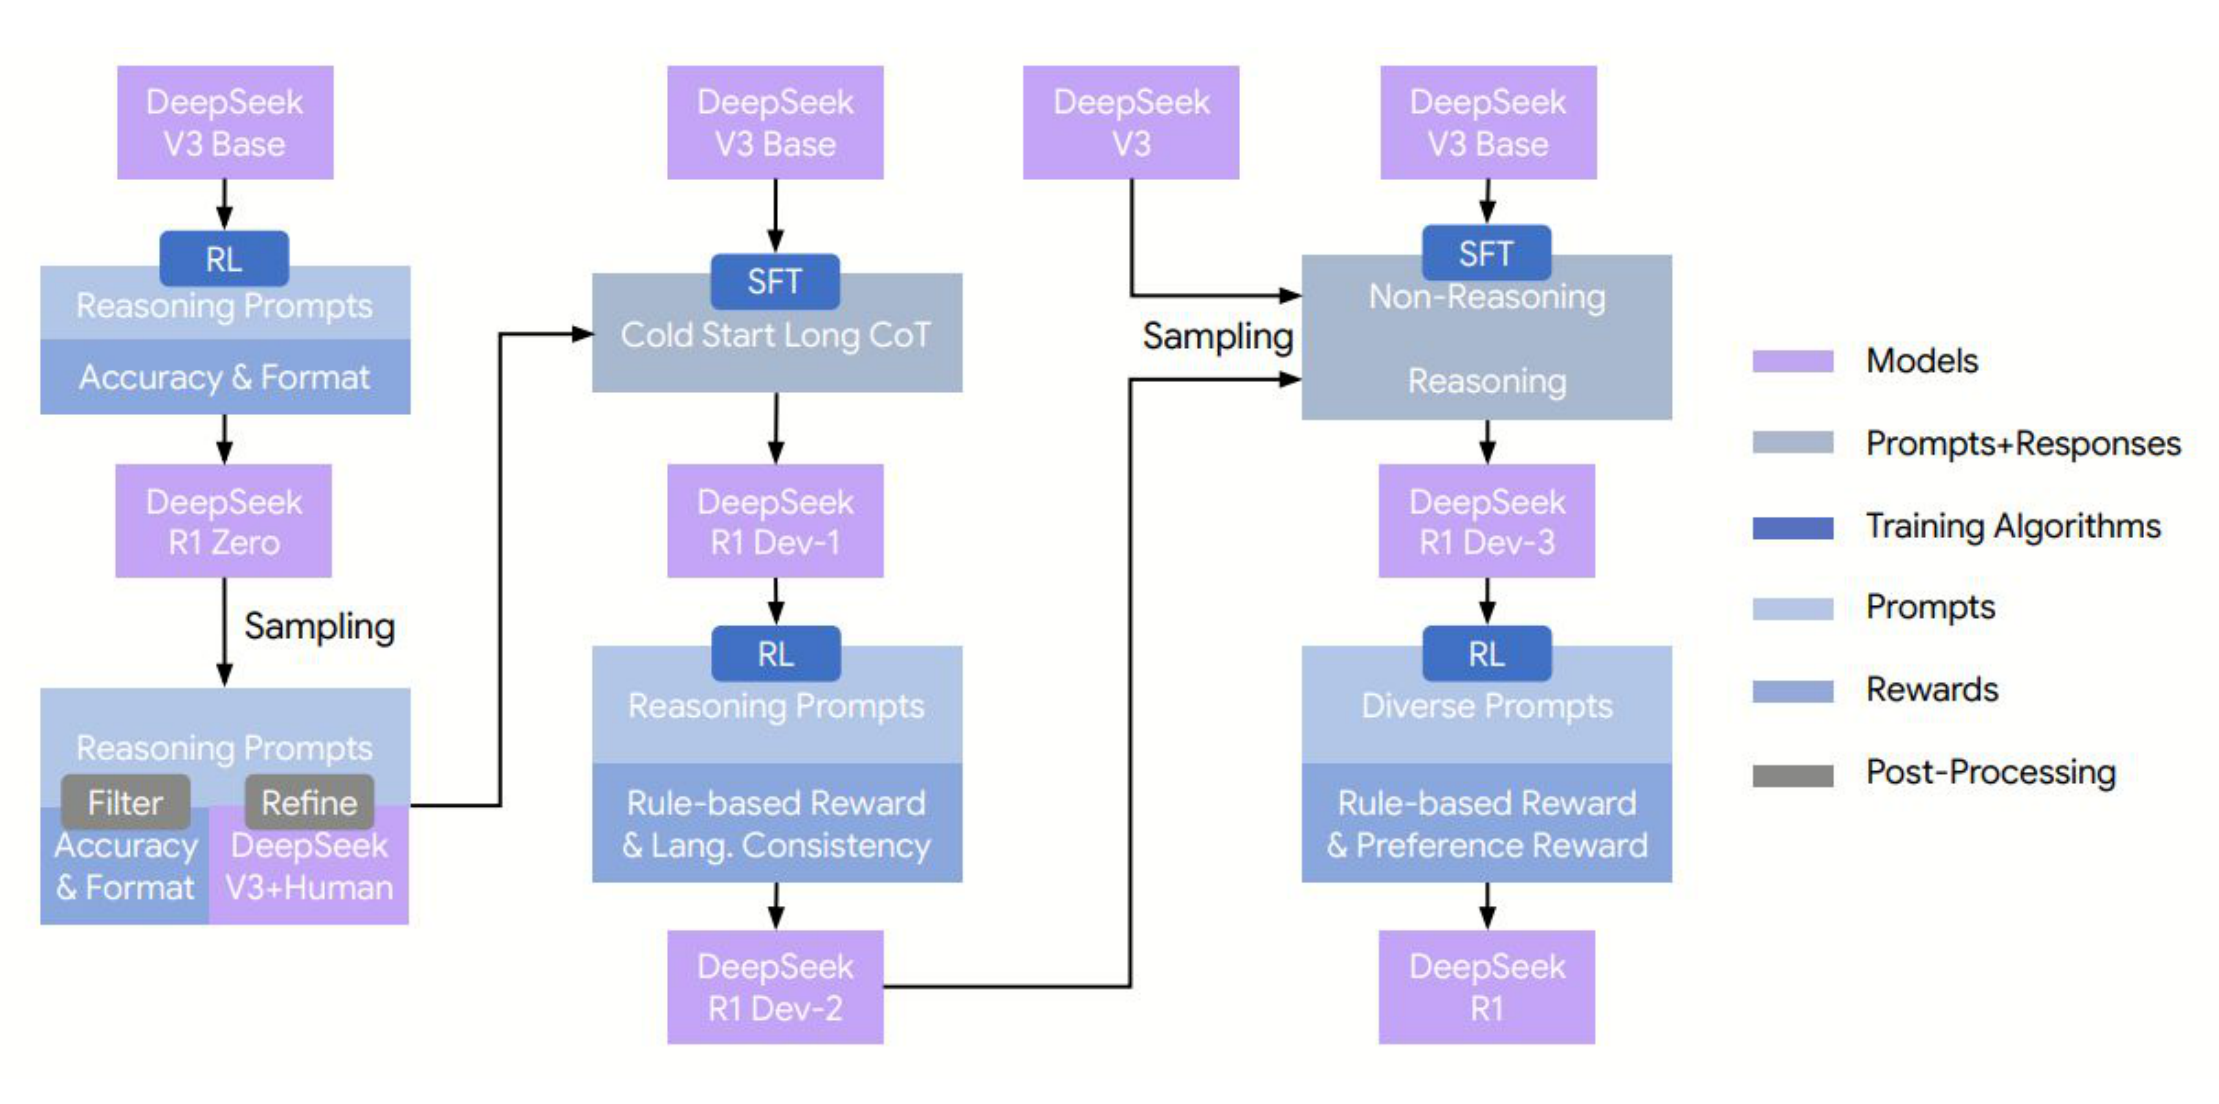
\includegraphics[width=\textwidth,height=0.86\textheight,keepaspectratio]{images/lrm-grpo/deepseek_r1_full_training_pipeline.png}
    \caption*{Source: DeepSeek-AI (2025), \href{https://arxiv.org/abs/2501.12948}{arXiv:2501.12948}, Fig.~2; via Stanford CS224N, Lecture 12 (Choi, 2026).}
  \end{figure}
\end{frame}

\begin{frame}{Key findings: DeepSeek-R1}
  \begin{itemize}
    \item<1-> \textcolor{KAred}{\textbf{Finding 1: RL alone can induce reasoning}}
    \begin{itemize}
      \item \textbf{Prior assumption}: chain-of-thought reasoning required supervised examples.
      \item \textbf{Finding}: R1-Zero demonstrates that outcome-based RL, with no process supervision, can induce sophisticated reasoning capabilities.
      \item \textbf{Caveat 1}: the final R1 is still going through the SFT$\rightarrow$RL pipeline in the end
      \item \textbf{Caveat 2}: doesn't apply to small (less capable) models
    \end{itemize}
  \end{itemize}
  \vfill
  {\scriptsize Findings 1--7 follow Stanford CS224N, Lecture 12 (Choi, 2026).}
\end{frame}

\begin{frame}{Key findings: DeepSeek-R1}
  \begin{itemize}
    \item<1-> \textcolor{KAred}{\textbf{Finding 2: Outcome rewards can enable discovery}}
    \begin{itemize}
      \item \textbf{Prior assumption}: sophisticated process rewards are necessary for O1 reasoning.
      \item \textbf{Finding}: Process reward models can inadvertently constrain exploration by penalizing unconventional yet effective reasoning paths. The lesson: sometimes less supervision yields more capability.
      \item \textbf{Caveat}: RLVR is not applicable for all reasoning problems.
    \end{itemize}
  \end{itemize}
\end{frame}

\begin{frame}{Key findings: DeepSeek-R1}
  \begin{itemize}
    \item<1-> \textcolor{KAred}{\textbf{Finding 3: RL + SFT synergy}}
    \begin{itemize}
      \item Neither pure RL (R1-Zero) nor pure SFT produces the best results.
      \item The multi-stage pipeline shows that RL and SFT play complementary roles: RL discovers capability, SFT provides reliability.
      \item Cold-start data prevents early RL instability; rejection sampling converts RL discoveries into reusable training data.
    \end{itemize}
  \end{itemize}
\end{frame}

\begin{frame}{Key findings: DeepSeek-R1}
  \begin{itemize}
    \item<1-> \textcolor{KAred}{\textbf{Finding 4: Distillation outperforms direct RL on small models}}
    \begin{itemize}
      \item If you have a limited compute budget, you are better off distilling from a large reasoning model than applying RL to a small model directly.
      \item Through distillation, reasoning capabilities transfer to models as small as 1.5B parameters, making strong reasoning accessible at any scale.
    \end{itemize}
    \item<2-> \textcolor{KAred}{\textbf{Finding 5: Open-weight reasoning models are viable}}
    \begin{itemize}
      \item R1 models are released under an MIT license.
      \item The distilled 7B and 14B models outperform many much larger closed-source models on reasoning benchmarks.
    \end{itemize}
  \end{itemize}
\end{frame}

\begin{frame}{Key findings}
  \begin{itemize}
    \item<1-> \textcolor{KAred}{\textbf{Finding 6: Structured search algorithms for inference scaling?}}\\
      \vspace{0.3em}
      \begin{itemize}
        \item \textbf{Prior assumption}: Inference-time search algorithm such as Monte-Carlo Tree Search might be necessary.
        \item \textbf{Findings}: Reasoning can be entirely autoregressive; no special search algorithm necessary.
        \item \textbf{Caveat}: Later models for hard math benchmarks do incorporate structure, though not in the traditional MCTS sense.
      \end{itemize}
  \end{itemize}
\end{frame}

\begin{frame}{Key findings: DeepSeek-R1}
  \begin{itemize}
    \item<1-> \textcolor{KAred}{\textbf{Finding 7: Test-time compute is a learnable resource}}
    \begin{itemize}
      \item \textbf{Findings}: R1's models learn to allocate more thinking tokens to harder problems. Test-time compute scaling is therefore more than an inference trick like beam search or majority voting; the model itself learns when and how much to think.
      \item \textbf{Caveat}: true to some degree; later studies reveal challenges to address.
    \end{itemize}
  \end{itemize}
\end{frame}
